\section*{\nr.4 \titfour (25 Punkte)}
\begin{enumerate}[(a)]
\item In die Formel für die relativistische Gesamtenergie
\begin{equation}
E = \sqrt{p^2c^2+m^2c^4}
\end{equation}
werden die Beziehungen $E=\hbar \omega$ und $p= \hbar k$ eingesetzt und nach $\omega$ aufgelöst. Dies führt direkt zur Dispersionsrelation:
\begin{equation}
\omega(k) = \sqrt{k^2c^2+\frac{m^2c^4}{\hbar^2}}
\label{eq:disp}
\end{equation}
\item Die Phasengeschwindigkeit errechnet sich zu:
\begin{equation}
v_\text{ph} = \frac{\omega}{k} = \sqrt{c^2+\frac{m^2c^4}{k^2\hbar^2}}
\end{equation}
Die Gruppengeschwindigkeit beträgt:
\begin{equation}
v_\text{gr} = \frac{\mathrm{d}\omega}{\mathrm{d}k} = \frac{c^2 k}{\sqrt{k^2c^2+\frac{m^2c^4}{\hbar^2}}}
\end{equation}
Abbildungen von Phasen- und Gruppengeschwindigkeit am Beispiel eines Elektrons sind durch \vref{fig:vphase,fig:vgruppe} gegeben.
\begin{figure}[htbp]
\centering
% GNUPLOT: LaTeX picture with Postscript
\begingroup
  \makeatletter
  \providecommand\color[2][]{%
    \GenericError{(gnuplot) \space\space\space\@spaces}{%
      Package color not loaded in conjunction with
      terminal option `colourtext'%
    }{See the gnuplot documentation for explanation.%
    }{Either use 'blacktext' in gnuplot or load the package
      color.sty in LaTeX.}%
    \renewcommand\color[2][]{}%
  }%
  \providecommand\includegraphics[2][]{%
    \GenericError{(gnuplot) \space\space\space\@spaces}{%
      Package graphicx or graphics not loaded%
    }{See the gnuplot documentation for explanation.%
    }{The gnuplot epslatex terminal needs graphicx.sty or graphics.sty.}%
    \renewcommand\includegraphics[2][]{}%
  }%
  \providecommand\rotatebox[2]{#2}%
  \@ifundefined{ifGPcolor}{%
    \newif\ifGPcolor
    \GPcolortrue
  }{}%
  \@ifundefined{ifGPblacktext}{%
    \newif\ifGPblacktext
    \GPblacktextfalse
  }{}%
  % define a \g@addto@macro without @ in the name:
  \let\gplgaddtomacro\g@addto@macro
  % define empty templates for all commands taking text:
  \gdef\gplbacktext{}%
  \gdef\gplfronttext{}%
  \makeatother
  \ifGPblacktext
    % no textcolor at all
    \def\colorrgb#1{}%
    \def\colorgray#1{}%
  \else
    % gray or color?
    \ifGPcolor
      \def\colorrgb#1{\color[rgb]{#1}}%
      \def\colorgray#1{\color[gray]{#1}}%
      \expandafter\def\csname LTw\endcsname{\color{white}}%
      \expandafter\def\csname LTb\endcsname{\color{black}}%
      \expandafter\def\csname LTa\endcsname{\color{black}}%
      \expandafter\def\csname LT0\endcsname{\color[rgb]{1,0,0}}%
      \expandafter\def\csname LT1\endcsname{\color[rgb]{0,1,0}}%
      \expandafter\def\csname LT2\endcsname{\color[rgb]{0,0,1}}%
      \expandafter\def\csname LT3\endcsname{\color[rgb]{1,0,1}}%
      \expandafter\def\csname LT4\endcsname{\color[rgb]{0,1,1}}%
      \expandafter\def\csname LT5\endcsname{\color[rgb]{1,1,0}}%
      \expandafter\def\csname LT6\endcsname{\color[rgb]{0,0,0}}%
      \expandafter\def\csname LT7\endcsname{\color[rgb]{1,0.3,0}}%
      \expandafter\def\csname LT8\endcsname{\color[rgb]{0.5,0.5,0.5}}%
    \else
      % gray
      \def\colorrgb#1{\color{black}}%
      \def\colorgray#1{\color[gray]{#1}}%
      \expandafter\def\csname LTw\endcsname{\color{white}}%
      \expandafter\def\csname LTb\endcsname{\color{black}}%
      \expandafter\def\csname LTa\endcsname{\color{black}}%
      \expandafter\def\csname LT0\endcsname{\color{black}}%
      \expandafter\def\csname LT1\endcsname{\color{black}}%
      \expandafter\def\csname LT2\endcsname{\color{black}}%
      \expandafter\def\csname LT3\endcsname{\color{black}}%
      \expandafter\def\csname LT4\endcsname{\color{black}}%
      \expandafter\def\csname LT5\endcsname{\color{black}}%
      \expandafter\def\csname LT6\endcsname{\color{black}}%
      \expandafter\def\csname LT7\endcsname{\color{black}}%
      \expandafter\def\csname LT8\endcsname{\color{black}}%
    \fi
  \fi
    \setlength{\unitlength}{0.0500bp}%
    \ifx\gptboxheight\undefined%
      \newlength{\gptboxheight}%
      \newlength{\gptboxwidth}%
      \newsavebox{\gptboxtext}%
    \fi%
    \setlength{\fboxrule}{0.5pt}%
    \setlength{\fboxsep}{1pt}%
\begin{picture}(7936.00,5102.00)%
    \gplgaddtomacro\gplbacktext{%
      \csname LTb\endcsname%
      \put(682,704){\makebox(0,0)[r]{\strut{}$0$}}%
      \put(682,1643){\makebox(0,0)[r]{\strut{}$5$}}%
      \put(682,2583){\makebox(0,0)[r]{\strut{}$10$}}%
      \put(682,3522){\makebox(0,0)[r]{\strut{}$15$}}%
      \put(682,4461){\makebox(0,0)[r]{\strut{}$20$}}%
      \put(814,484){\makebox(0,0){\strut{}$0$}}%
      \put(2037,484){\makebox(0,0){\strut{}$2$}}%
      \put(3259,484){\makebox(0,0){\strut{}$4$}}%
      \put(4482,484){\makebox(0,0){\strut{}$6$}}%
      \put(5705,484){\makebox(0,0){\strut{}$8$}}%
      \put(6928,484){\makebox(0,0){\strut{}$10$}}%
    }%
    \gplgaddtomacro\gplfronttext{%
      \csname LTb\endcsname%
      \put(176,2770){\rotatebox{-270}{\makebox(0,0){\strut{}$v_{\text{ph}}$ in $10^{12}\,\si{\meter\per\second}$}}}%
      \put(4176,154){\makebox(0,0){\strut{}$k$ in $10^8\,\si{\meter}$}}%
    }%
    \gplgaddtomacro\gplbacktext{%
      \csname LTb\endcsname%
      \put(682,704){\makebox(0,0)[r]{\strut{}$0$}}%
      \put(682,1643){\makebox(0,0)[r]{\strut{}$5$}}%
      \put(682,2583){\makebox(0,0)[r]{\strut{}$10$}}%
      \put(682,3522){\makebox(0,0)[r]{\strut{}$15$}}%
      \put(682,4461){\makebox(0,0)[r]{\strut{}$20$}}%
      \put(814,484){\makebox(0,0){\strut{}$0$}}%
      \put(2037,484){\makebox(0,0){\strut{}$2$}}%
      \put(3259,484){\makebox(0,0){\strut{}$4$}}%
      \put(4482,484){\makebox(0,0){\strut{}$6$}}%
      \put(5705,484){\makebox(0,0){\strut{}$8$}}%
      \put(6928,484){\makebox(0,0){\strut{}$10$}}%
    }%
    \gplgaddtomacro\gplfronttext{%
      \csname LTb\endcsname%
      \put(176,2770){\rotatebox{-270}{\makebox(0,0){\strut{}$v_{\text{ph}}$ in $10^{12}\,\si{\meter\per\second}$}}}%
      \put(4176,154){\makebox(0,0){\strut{}$k$ in $10^8\,\si{\meter}$}}%
    }%
    \gplbacktext
    \put(0,0){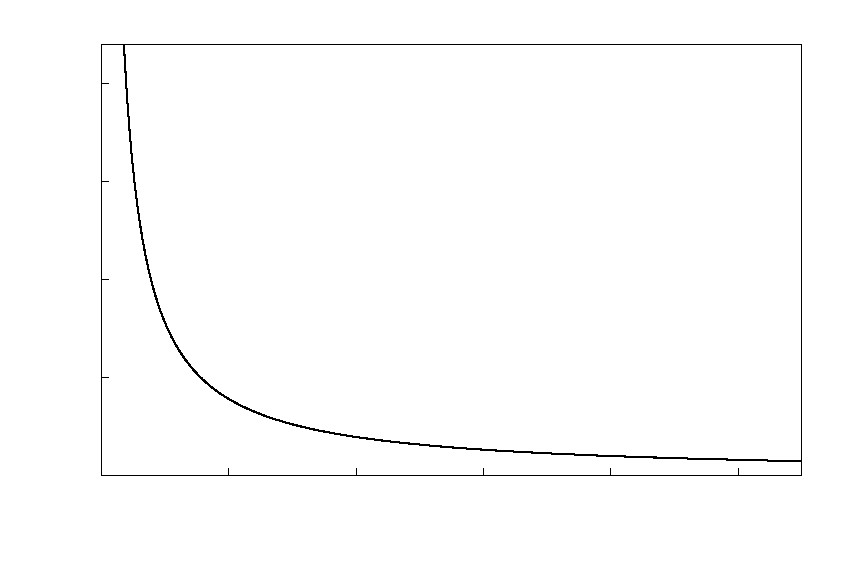
\includegraphics{vphase}}%
    \gplfronttext
  \end{picture}%
\endgroup

\caption{Phasengeschwindigkeit eines Elektrons. Ansatzweise ist zu erkennen, dass $v_\text{ph}=c$ eine waagrechte Asymptote des Graphen darstellt.}
\label{fig:vphase}
\end{figure}

\begin{figure}[htbp]
\centering
% GNUPLOT: LaTeX picture with Postscript
\begingroup
  \makeatletter
  \providecommand\color[2][]{%
    \GenericError{(gnuplot) \space\space\space\@spaces}{%
      Package color not loaded in conjunction with
      terminal option `colourtext'%
    }{See the gnuplot documentation for explanation.%
    }{Either use 'blacktext' in gnuplot or load the package
      color.sty in LaTeX.}%
    \renewcommand\color[2][]{}%
  }%
  \providecommand\includegraphics[2][]{%
    \GenericError{(gnuplot) \space\space\space\@spaces}{%
      Package graphicx or graphics not loaded%
    }{See the gnuplot documentation for explanation.%
    }{The gnuplot epslatex terminal needs graphicx.sty or graphics.sty.}%
    \renewcommand\includegraphics[2][]{}%
  }%
  \providecommand\rotatebox[2]{#2}%
  \@ifundefined{ifGPcolor}{%
    \newif\ifGPcolor
    \GPcolortrue
  }{}%
  \@ifundefined{ifGPblacktext}{%
    \newif\ifGPblacktext
    \GPblacktextfalse
  }{}%
  % define a \g@addto@macro without @ in the name:
  \let\gplgaddtomacro\g@addto@macro
  % define empty templates for all commands taking text:
  \gdef\gplbacktext{}%
  \gdef\gplfronttext{}%
  \makeatother
  \ifGPblacktext
    % no textcolor at all
    \def\colorrgb#1{}%
    \def\colorgray#1{}%
  \else
    % gray or color?
    \ifGPcolor
      \def\colorrgb#1{\color[rgb]{#1}}%
      \def\colorgray#1{\color[gray]{#1}}%
      \expandafter\def\csname LTw\endcsname{\color{white}}%
      \expandafter\def\csname LTb\endcsname{\color{black}}%
      \expandafter\def\csname LTa\endcsname{\color{black}}%
      \expandafter\def\csname LT0\endcsname{\color[rgb]{1,0,0}}%
      \expandafter\def\csname LT1\endcsname{\color[rgb]{0,1,0}}%
      \expandafter\def\csname LT2\endcsname{\color[rgb]{0,0,1}}%
      \expandafter\def\csname LT3\endcsname{\color[rgb]{1,0,1}}%
      \expandafter\def\csname LT4\endcsname{\color[rgb]{0,1,1}}%
      \expandafter\def\csname LT5\endcsname{\color[rgb]{1,1,0}}%
      \expandafter\def\csname LT6\endcsname{\color[rgb]{0,0,0}}%
      \expandafter\def\csname LT7\endcsname{\color[rgb]{1,0.3,0}}%
      \expandafter\def\csname LT8\endcsname{\color[rgb]{0.5,0.5,0.5}}%
    \else
      % gray
      \def\colorrgb#1{\color{black}}%
      \def\colorgray#1{\color[gray]{#1}}%
      \expandafter\def\csname LTw\endcsname{\color{white}}%
      \expandafter\def\csname LTb\endcsname{\color{black}}%
      \expandafter\def\csname LTa\endcsname{\color{black}}%
      \expandafter\def\csname LT0\endcsname{\color{black}}%
      \expandafter\def\csname LT1\endcsname{\color{black}}%
      \expandafter\def\csname LT2\endcsname{\color{black}}%
      \expandafter\def\csname LT3\endcsname{\color{black}}%
      \expandafter\def\csname LT4\endcsname{\color{black}}%
      \expandafter\def\csname LT5\endcsname{\color{black}}%
      \expandafter\def\csname LT6\endcsname{\color{black}}%
      \expandafter\def\csname LT7\endcsname{\color{black}}%
      \expandafter\def\csname LT8\endcsname{\color{black}}%
    \fi
  \fi
    \setlength{\unitlength}{0.0500bp}%
    \ifx\gptboxheight\undefined%
      \newlength{\gptboxheight}%
      \newlength{\gptboxwidth}%
      \newsavebox{\gptboxtext}%
    \fi%
    \setlength{\fboxrule}{0.5pt}%
    \setlength{\fboxsep}{1pt}%
\begin{picture}(7936.00,5102.00)%
    \gplgaddtomacro\gplbacktext{%
      \csname LTb\endcsname%
      \put(682,704){\makebox(0,0)[r]{\strut{}$0$}}%
      \put(682,1330){\makebox(0,0)[r]{\strut{}$5$}}%
      \put(682,1956){\makebox(0,0)[r]{\strut{}$10$}}%
      \put(682,2583){\makebox(0,0)[r]{\strut{}$15$}}%
      \put(682,3209){\makebox(0,0)[r]{\strut{}$20$}}%
      \put(682,3835){\makebox(0,0)[r]{\strut{}$25$}}%
      \put(682,4461){\makebox(0,0)[r]{\strut{}$30$}}%
      \put(814,484){\makebox(0,0){\strut{}$0$}}%
      \put(2735,484){\makebox(0,0){\strut{}$2$}}%
      \put(4657,484){\makebox(0,0){\strut{}$4$}}%
      \put(6578,484){\makebox(0,0){\strut{}$6$}}%
    }%
    \gplgaddtomacro\gplfronttext{%
      \csname LTb\endcsname%
      \put(176,2770){\rotatebox{-270}{\makebox(0,0){\strut{}$v_{\text{gr}}$ in $10^{7}\,\si{\meter\per\second}$}}}%
      \put(4176,154){\makebox(0,0){\strut{}$k$ in $10^{13}\,\si{\meter}$}}%
    }%
    \gplgaddtomacro\gplbacktext{%
      \csname LTb\endcsname%
      \put(682,704){\makebox(0,0)[r]{\strut{}$0$}}%
      \put(682,1330){\makebox(0,0)[r]{\strut{}$5$}}%
      \put(682,1956){\makebox(0,0)[r]{\strut{}$10$}}%
      \put(682,2583){\makebox(0,0)[r]{\strut{}$15$}}%
      \put(682,3209){\makebox(0,0)[r]{\strut{}$20$}}%
      \put(682,3835){\makebox(0,0)[r]{\strut{}$25$}}%
      \put(682,4461){\makebox(0,0)[r]{\strut{}$30$}}%
      \put(814,484){\makebox(0,0){\strut{}$0$}}%
      \put(2735,484){\makebox(0,0){\strut{}$2$}}%
      \put(4657,484){\makebox(0,0){\strut{}$4$}}%
      \put(6578,484){\makebox(0,0){\strut{}$6$}}%
    }%
    \gplgaddtomacro\gplfronttext{%
      \csname LTb\endcsname%
      \put(176,2770){\rotatebox{-270}{\makebox(0,0){\strut{}$v_{\text{gr}}$ in $10^{7}\,\si{\meter\per\second}$}}}%
      \put(4176,154){\makebox(0,0){\strut{}$k$ in $10^{13}\,\si{\meter}$}}%
    }%
    \gplbacktext
    \put(0,0){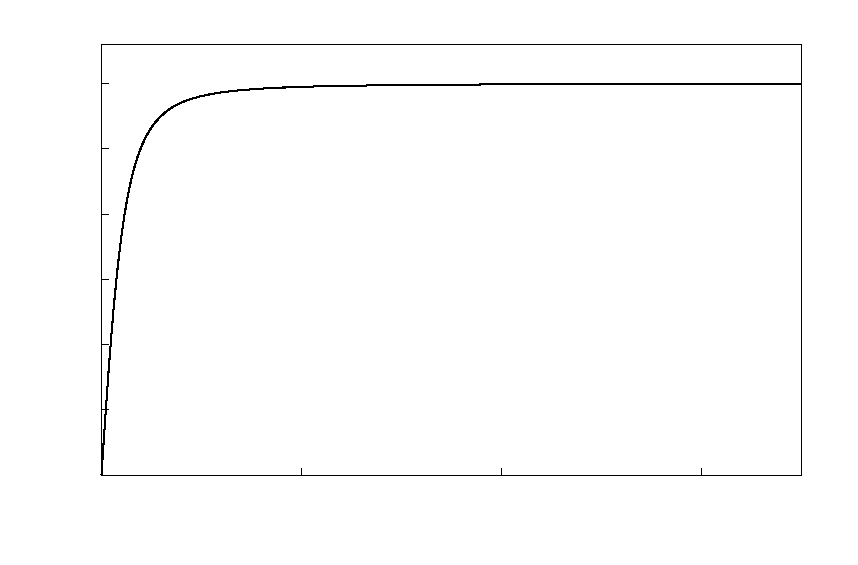
\includegraphics{vgruppe}}%
    \gplfronttext
  \end{picture}%
\endgroup

\caption{Gruppengeschwindigkeit eines Elektrons. Ansatzweise ist zu erkennen, dass $v_\text{ph}=c$ eine waagrechte Asymptote des Graphen darstellt.}
\label{fig:vgruppe}
\end{figure}
\item Das Produkt dieser beiden Geschwindigkeiten beträgt
\begin{equation}
v_\text{ph}\cdot v_\text{gr} = \frac{1}{k}\sqrt{k^2c^2+\frac{m^2c^4}{\hbar^2}} \frac{c^2 k}{\sqrt{k^2c^2+\frac{m^2c^4}{\hbar^2}}} = c^2,
\end{equation}
ist also unabhängig von $k$ konstant.
\item  Führt man den obigen Formalismus für $E(p) = p^2/(2m) + mc^2$ durch, so erhält man die Dispersionsrelation
\begin{equation}
\omega = \frac{\hbar k^2}{2m} +\frac{mc^2}{\hbar} = \frac{c k^2}{2k_C} +ck_C
\end{equation}
mit $k_C = mc/\hbar$. Diese Relation erhält man jedoch auch aus \vref{eq:disp} durch eine Taylor-Entwicklung um $k=0$: Es gilt:
\begin{align}
\frac{1}{ck_C}\omega(0) &= 1 \\
\frac{1}{ck_C} \frac{\mathrm{d}\omega}{\mathrm{d}k}(0) &= \left. \frac{k/k_C^2}{\sqrt{1+k^2/k_C^2}}\right|_{k=0} = 0 \\
\frac{1}{ck_C} \frac{\mathrm{d}^2\omega}{\mathrm{d}k^2}(0) &= \frac{1}{k_C^2}
\end{align}
Die Taylor-Entwicklung bis zur zweiten Ordnung ergibt somit:
\begin{equation}
\omega(k) = ck_C \left( 1 + \frac{k^2}{2k_C^2} + \mathcal{O}(k^4) \right)
\end{equation}
Das deckt sich mit der klassischen Erwartung.
\item Wellenpakete werden relativistisch bei großen Impulsen, also großen $k$. Die klassische Dispersionsrelation ist quadratisch in $k$, während die relativistische Dispersionsrelation für große $k$ nur linear mit $k$ wächst. Somit zeigen relativistische Wellenpakete weniger Dispersion.
\item Der ultrarelativistische Grenzfall kann nur mit verschwindender Ruhemasse $m$ erreicht werden. In diesem Fall reduziert sich die relativistische Dispersionsrelation~(\ref{eq:disp}) zu:
\begin{equation}
\omega(k) = kc
\end{equation}
Die Gruppen- (und auch die Phasen-) Geschwindigkeit hängen dann nicht mehr von $k$ ab, somit gibt es keine Dispersion.
\end{enumerate}